\documentclass[12pt,a4paper]{article}
\usepackage[utf8]{inputenc}
\usepackage[brazil]{babel}
\usepackage{graphicx}
\usepackage{amssymb, amsfonts, amsmath}
\usepackage{float}
\usepackage{enumerate}
\usepackage[top=2.5cm, bottom=2.5cm, left=1.25cm, right=1.25cm]{geometry}

\begin{document}
\pagestyle{empty}

\begin{center}
  \begin{tabular}{ccc}
    \begin{tabular}{c}
      \includegraphics[scale=0.25]{../../biblioteca/imagem/brasao-de-armas-brasil} \\
    \end{tabular} & 
    \begin{tabular}{c}
      Ministério da Educação \\
      Universidade Federal dos Vales do Jequitinhonha e Mucuri \\
      Faculdade de Ciências Sociais, Aplicadas e Exatas - FACSAE \\
      Departamento de Ciências Exatas - DCEX \\
      Disciplina: Matemática Elementar I \quad Semestre: 2021/1\\
      Prof. Me. Luiz C. M. de Aquino\\
    \end{tabular} &
    \begin{tabular}{c}
      \includegraphics[scale=0.25]{../../biblioteca/imagem/logo-ufvjm} \\
    \end{tabular}
  \end{tabular}
\end{center}

\begin{center}
  \textbf{Lista V}
\end{center}

\begin{enumerate}
  \item Determine a função $f$ polinomial do 2° grau tal que seu gráfico passa
  pelos pontos $(-1,\,4)$, $(1,\,-6)$ e $(2,\,-5)$.
  
  \item Considere que $f$ é uma função polinomial do 2° grau, cujo o gráfico está
  ilustrado abaixo. Determine os pontos que esse gráfico corta o eixo $x$.

  \begin{figure}[H]
   \centering
   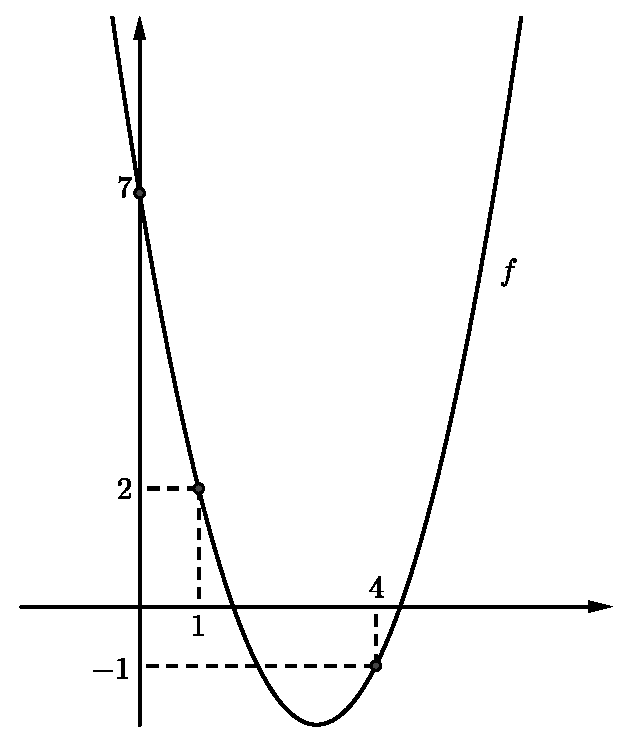
\includegraphics[scale=0.625]{figura/grafico-funcao-polinomio-segundo-grau.eps}
  \end{figure}

  \item Determine o domínio das funções definidas abaixo.
  \begin{enumerate}
    \item $f(x) = \dfrac{\sqrt{-x^2 + 6x - 8}}{x - 2}$.
    \item $g(x) = \dfrac{\sqrt{-x^2 + 2x} - \sqrt{x^2 - 4x + 3}}{x - 1}$. 
  \end{enumerate}

  \item (ENEM 2014 - Adaptada) Um professor, depois de corrigir as provas de sua turma, percebeu que várias questões estavam 
 muito difíceis. Para compensar, decidiu utilizar uma função polinomial $f$, de grau menor que 3, para alterar as notas $x$ da prova para notas $y = f(x)$, 
 da seguinte maneira:
 
 \begin{itemize}
  \item a nota zero permanece zero;
  \item a nota 10 permanece 10;
  \item a nota 5 passa a ser 6.
 \end{itemize}

 Determine a expressão de $y = f(x)$ a ser utilizada pelo professor.
  
  \item Suponha que $f$ seja uma função polinomial do 2° grau tal que
  $f(0) = p$, $f\left(\dfrac{1}{2}\right) = q$ e $f(1) = r$. Prove 
  que $f(x) = 2(1 - x)\left(\dfrac{1}{2} - x\right)p + 4x(1 - x)q - 2x\left(\dfrac{1}{2} - x\right)r$.

\end{enumerate}

\begin{center}
  \textbf{Gabarito}
\end{center}

[1] $f(x) = 2x^2 - 5x - 3$.
[2] $x = 3 - \sqrt{2}$ e $x = 3 + \sqrt{2}$.
[3] 
(a) $D = \left\{x\in \mathbb{R}\,|\, 2 < x \leq 4\right\}$. 
(b) $D = \left\{x\in \mathbb{R}\,|\, 0 \leq x < 1\right\}$. 
[4] $y = -\dfrac{1}{25}x^2 + \dfrac{7}{5}x$. 
[5] Sugestão: considerando que $f(x) = ax^2 + bx + c$, resolva o sistema de equações formado por 
$f(0) = p$, $f\left(\dfrac{1}{2}\right) = q$ e $f(1) = r$.  

\end{document}